\chapter{Понятие нейронных сетей, их классификация, основные области применения}
Началом понятия нейронной сети послужила биологическая модель нейрона человеческого мозга.
Уорреном МакКаллокм (Warren McCulloch) и Уолтер Питтс (Walter Pitts) в 1943 году предложили
модель искусственного нейрона, которая получила название перцептрон. Перцептрон принимал на вход $n$ бинарных величин $x_1, \dots x_n$,
которые учитываются с весами $w_1, \dots, w_n$. На основе значения, полученного сумматором $\sum_{i=1}^n x_i w_i$, функция активации
$\varphi$ формирует выходное значение $a$, которое определяется по формуле:
\begin{equation}
    a = \varphi \left( \sum\limits_{i=1}^n x_i w_i \right).
\end{equation}

\begin{figure}[H]
	\center{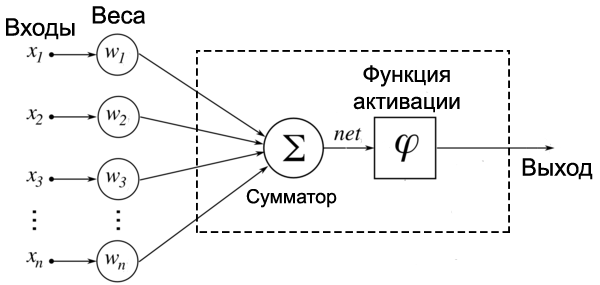
\includegraphics[width=0.7\linewidth]{img/perceptron.png}}
	\caption{Перцептрон}
\end{figure}

Упомянутые ученые также предложили способ объединения искусственных нейронов в сети, называемые нейронными сетями.
Нейроны, находящиеся на одном уровне обработки входных данных, объединялись в слои.
Слой, который принимает сигналы из внешнего мира, называется входным. Слой, который выдает сигналы во внешний мир, —
выходным. Остальные слои называются скрытыми \cite{sozykin}.

Процесс подбора весов называется процессом обучения нейросети.
Обучение происходит на уже имеющемся наборе входных данных и
решений: веса нейросети подбираются так, чтобы в среднем для всей
обучающей выборки ошибка в выходных данных и действительного
решения была минимальна \cite{cyber_alex}.

Для решения задачи необходимо выбрать определенный набор
нейронов и правильно их соединить. Рабочие модели нейросетей
насчитывают от сотен тысяч до десятков и сотен миллионов нейронов.
Однако отдельные нейроны не используются в составлении нейросетей изза сложности практических задач. Вместо этого используют специальные
наборы с заранее известной структурой. Их называют слоями, а из них в
свою очередь составляются сложные большие нейронные сети, пригодные
для решения задач. Общий вид, или структура, нейросети со всеми слоями,
функциями активации, регуляризации, входными и выходными нейронами
называется архитектурой нейросети \cite{cyber_alex}.

Нейронные сети можно классифицировать в зависимости от различных качеств.
1. По характеру обучения

С учителем, когда известно выходное пространство решений нейронной сети, а также предполагается, что имеются входные сигналы и
эталонные реакции на них. В процессе обучения происходит целенаправленная модификация синаптических связей нейронной сети (NN)
для достижения наилучшего соответствия между реальными выходными значениями сети Y и их эталонными значениями.

Без учителя. В этом случае нейронная сеть формирует выходное
пространство решений только на основе входных воздействий. Такие
сети называются самоорганизующимися

Подкрепляющее обучение (reinforcement learning). Происходит на основе сигнала подкрепления r от внешней среды.

Рекуррентные нейронные сети -- подкласс нейронных сетей с обратными связями, которые
используют предыдущие состояния сети для вычисления текущего. Сеть строится из узлов, каждый
из которых соединѐн со всеми другими узлами. У каждого нейрона порог активации меняется со
временем и является вещественным числом \cite{bguir_rnn}. 
Рекуррентные нейронные сети применяются для прогнозирования временных процессов \cite{bgu_krasn}, анализа естественного языка и других задач.
\begin{figure}[H]
	\center{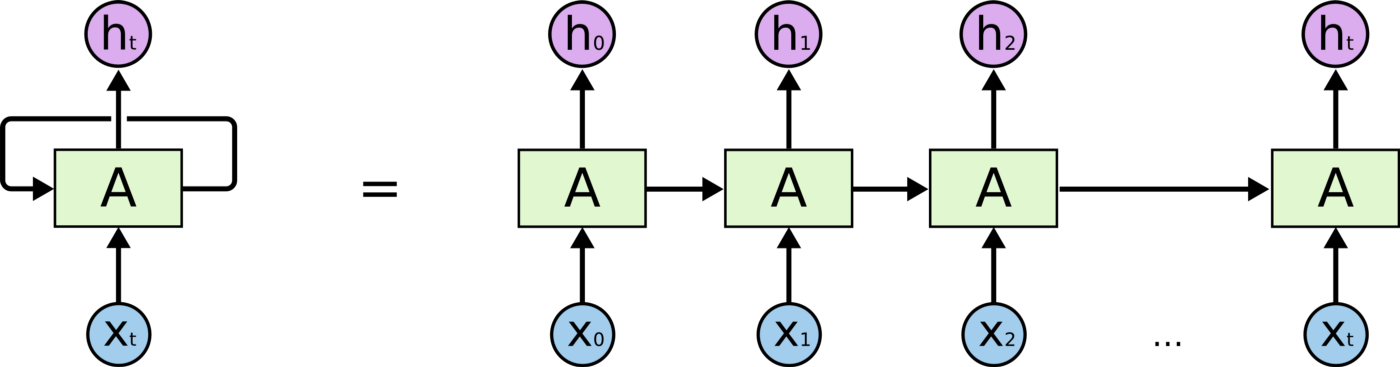
\includegraphics[width=0.7\linewidth]{img/rnn.png}}
	\caption{Иллюстрация работы рекуррентной нейронной сети}
\end{figure}

Автоэнкодерные сети -- подкласс нейронных сетей, для которых характерно наличие сжимающего слоя (энкодера) и восстанавлювающего словя (декодeра).
В процессе вычислений размерность входных данных данных понижается, над которыми далее могут производиться дополнительные преобразования, 
после чего размерность сжатых данных (латентного вектора) повышается \cite{vae}.
\begin{figure}[H]
	\center{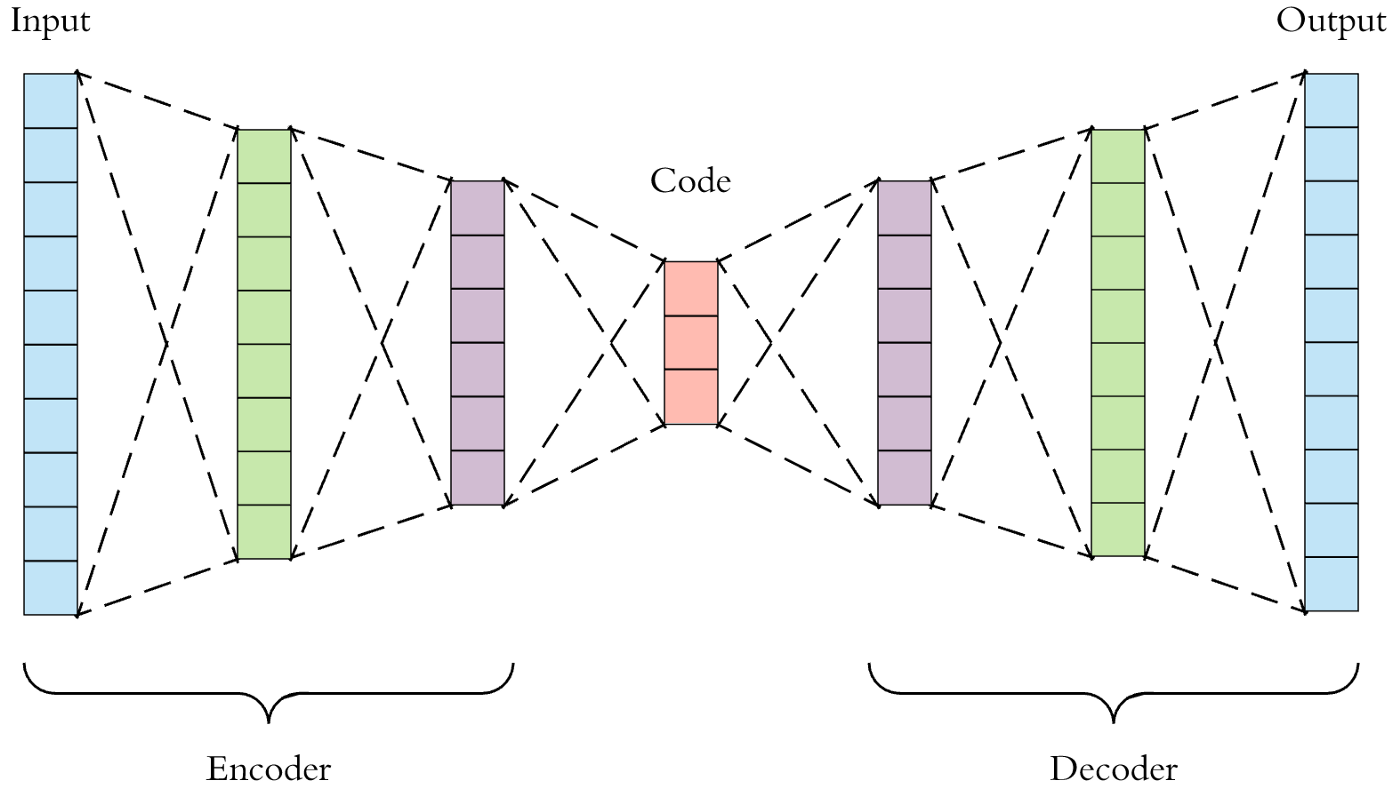
\includegraphics[width=0.7\linewidth]{img/autoencoder.png}}
	\caption{Иллюстрация работы автоэнкодера}
\end{figure}

Автоэнкодерные нейронные сети применяются для выделения наиболее важных информативных признаков 
(feature extraction) во входном пространстве образов, сжатия информации, очистки
данных от шумов, визуализации и классификации данных \cite{bgu_krasn}.
Данные нейронные сети нашли широкое применение в задачах генерации образов как составляющая генеративно-состязательных сетей.

Также выделяют самоорганизующиеся нейронные сети (self-organising neural networks), которые характеризуются обучением без учителя, в результате которого происходит адаптация сети к решаемой задаче . Их разработал в 80-е гг. XX в.
финский ученый Т. Кохонен (T. Kohonen). Нейронные сети
Кохонена осуществляют топологическое упорядочивание входного
пространства образов, поступающих на сеть. Они широко применяются
в задачах распознавания и визуализации образов, оптимизации и
управления. Одним из важных применений самоорганизующихся нейронных сетей является решение задачи коммивояжера.

\chapter{Основные методы анализа аудиоданных. Анализ аудиоданных при помощи нейросетевых методов}
Аудиоданные многомерны, содержат информацию о частотах закодированного звука с 
определенной периодичностью. 

Зачастую в аудиоданных присутствуют искажения, образцы характеризуются разным качеством звука и различной продолжительностью. 
Таким образом, GTZAN, один из самых популярных наборов данных, используемых в задачах анализа, идентификации и классификации аудиоданных по
звуковым данным (противопоставляется задаче анализа аудиоданных по содержанию метаданных), критикуется за различный битрейт композиций, которые входят в его состав \cite{gtzan}.
Поэтому к исходным данным применяют преобразования, которые убирают шумы и выделяют из данных самые важные характеристики.

Классическим средством обработки звука является преобразование Фурье $\mathcal{F}$ сигнала $f(t)$, вычисляемое по формуле:
\begin{equation} \label{eq:ft}
	F(\omega) = \int_{-\infty}^{+\infty} f(t) e ^ {-i \omega t} dt
\end{equation} и обратное ему преобразование -- обратное преобразование Фурье:
\begin{equation}
	f(t) = \frac{1}{2\pi} \int_{-\infty}^{+\infty} F(\omega) e^{-i \omega t} d\omega
\end{equation}

На практике вычисление (\ref{eq:ft}) затруднительно, поэтому используется быстрое дискретное преобразование Фурье дискретного сигнала $\left\{x_n\right\}$, вычисляемое по формуле:
\begin{equation}
	X_k = \sum_{n=0}^{N-1} x_n \cdot e^\frac{-2\pi i kn}{N}, k=\overline{0, N-1},
\end{equation}
где $e^{\frac{2\pi i}{N}}$ -- $N$-ый простой корень из $1$.

Сложность вычисления дискретного преобразования Фурье от сигнала размерности $N$ занимает $O(N^2)$ операций, что может стать проблемой при обработке
данных высокой размерности, так что зачастую применяется модификация данного преобразования, позволяющая получить аналогичный результат
за $O(N\log N )$ операций, например, с помощью алгоритма Кули — Тьюки, который является один из самых распространненых \cite{fft}.

Однако, сигнал, обработанный преобразованием Фурье, раскладывается по особым гармоникам -- волнам с частотой, которая кратна величине, обратной периоду, что далеко от восприятия человеческого уха.
Поэтому такой сигнал имеет смысл дополнительно обработать, чтобы он соответствовал человеческим представлением о музыке и звуке \cite{cyber_zub}.

Примером такой обработки аудиоданных является вейвлет-преобразование.
Вейвлет-преобразование — интегральное преобразование, которое представляет собой свертку вейвлет-функции с сигналом.
Вейвлет-преобразование переводит сигнал из временного представления в частотно-временное, что может быть удобно при выделении характеристик
в аудиоданных. Если исходный сигнал $\psi(t)$ непрерывен, то непрерывное вейвлет-преобразование может определяться
следующим образом:
\begin{equation}
	T(a,b)={\frac {1}{{\sqrt {a}}}}\int \limits _{{-\infty }}^{{\infty }}x(t)\psi ^{*}\left({\frac {t-b}{a}}\right)\,dt,
\end{equation} где
${\psi }^{*}$ означает комплексное сопряжение для $\psi$ , параметр $b\in \mathbb{R}$ соответствует временному сдвигу, 
и называется параметром положения, параметр $a > 0$ задает масштабирование и называется параметром растяжения, а множитель  $w(a) = \frac{1}{\sqrt{a}}$ отвечает за нормировку.

Аналогичным образом вводится и дискретное вейвлет-преобразование.
В дискретном случае параметры масштабирования a и сдвига b являются дискретными величинами:

$$a=a_{0}^{m},\quad b=nb_{0}$$

Тогда анализирующий вейвлет имеет следующий вид:

\begin{equation}
	\psi _{{m,n}}=a_{0}^{{-m/2}}\psi \left({\frac {t-nb_{0}}{a_{0}^{m}}}\right),
\end{equation}

где $m$ и $n$— целые числа.

Итого, дискретное вейвлет-преобразование и его обратное преобразование переписываются следующим образом:
\begin{equation}
	T_{{m,n}}=\int \limits _{{-\infty }}^{{\infty }}x(t)\,\psi _{{m,n}}^{*}(t)\,dt
\end{equation}

Величины $T_{{m,n}}$ также известны как вейвлет-коэффициенты.

В дискретном вейвлет-преобразовании наиболее значимая информация в сигнале содержится при высоких амплитудах, а менее значимая -- при низких.
Сжатие данных может быть получено за счет отбрасывания низких амплитуд.
Вейвлет-преобразование позволяет получить высокое соотношение сжатия в сочетании с хорошим качеством восстановленного сигнала. 
Вейвлет-преобразование было выбрано для стандартов сжатия изображений JPEG2000 и ICER.
Однако, при малых сжатиях вейвлет-преобразование уступает по качеству в сравнении с оконным Фурье-преобразованием, которое лежит в основе стандарта JPEG \cite{wavelet}. 

Примером характеристик, получаемых с использованием вышеупомянутых преобразований, служат мел-кепстральные коэффициенты (Mel-frequency cepstral coefficients) -- MFCC,
спектральные плотности мощности сигнала в каждый момент времени, 
спектральные полосы, хроматограммы по форме сигнала или по спектрограмме мощности и так далее \cite{mus_zhao}.

Спектральная плотность мощности $S(\omega)$ сигнала $x(t)$ на промежутке времени $\left[-\frac{T}{2},\frac{T}{2}\right]$ расчитывается как:
\begin{equation}
	S(\omega) = \lim_{T->+\infty} \frac{\left|F_T(\omega)\right|^2}{T},
\end{equation}
где
\begin{equation}
	F_{T}(\omega )={\frac {1}{\sqrt {2\pi }}}\int \limits _{-T/2}^{T/2}x(t)e^{-i\omega t} dt
\end{equation}
-- преобразование Фурье	от $x(t)$ \cite{otnes}.

Зависимость спектральной плотности мощности сигнала от времени характеризуют через изображения -- спектрограммы.
Наиболее распространенным представлением спектрограммы является двумерная диаграмма: на горизонтальной оси представлено время, 
по вертикальной оси — частота; третье измерение с указанием амплитуды на определенной частоте в конкретный момент времени представлено 
интенсивностью или цветом каждой точки изображения (Рисунок \ref{fig:spec}).

\begin{figure}[H]
	\center{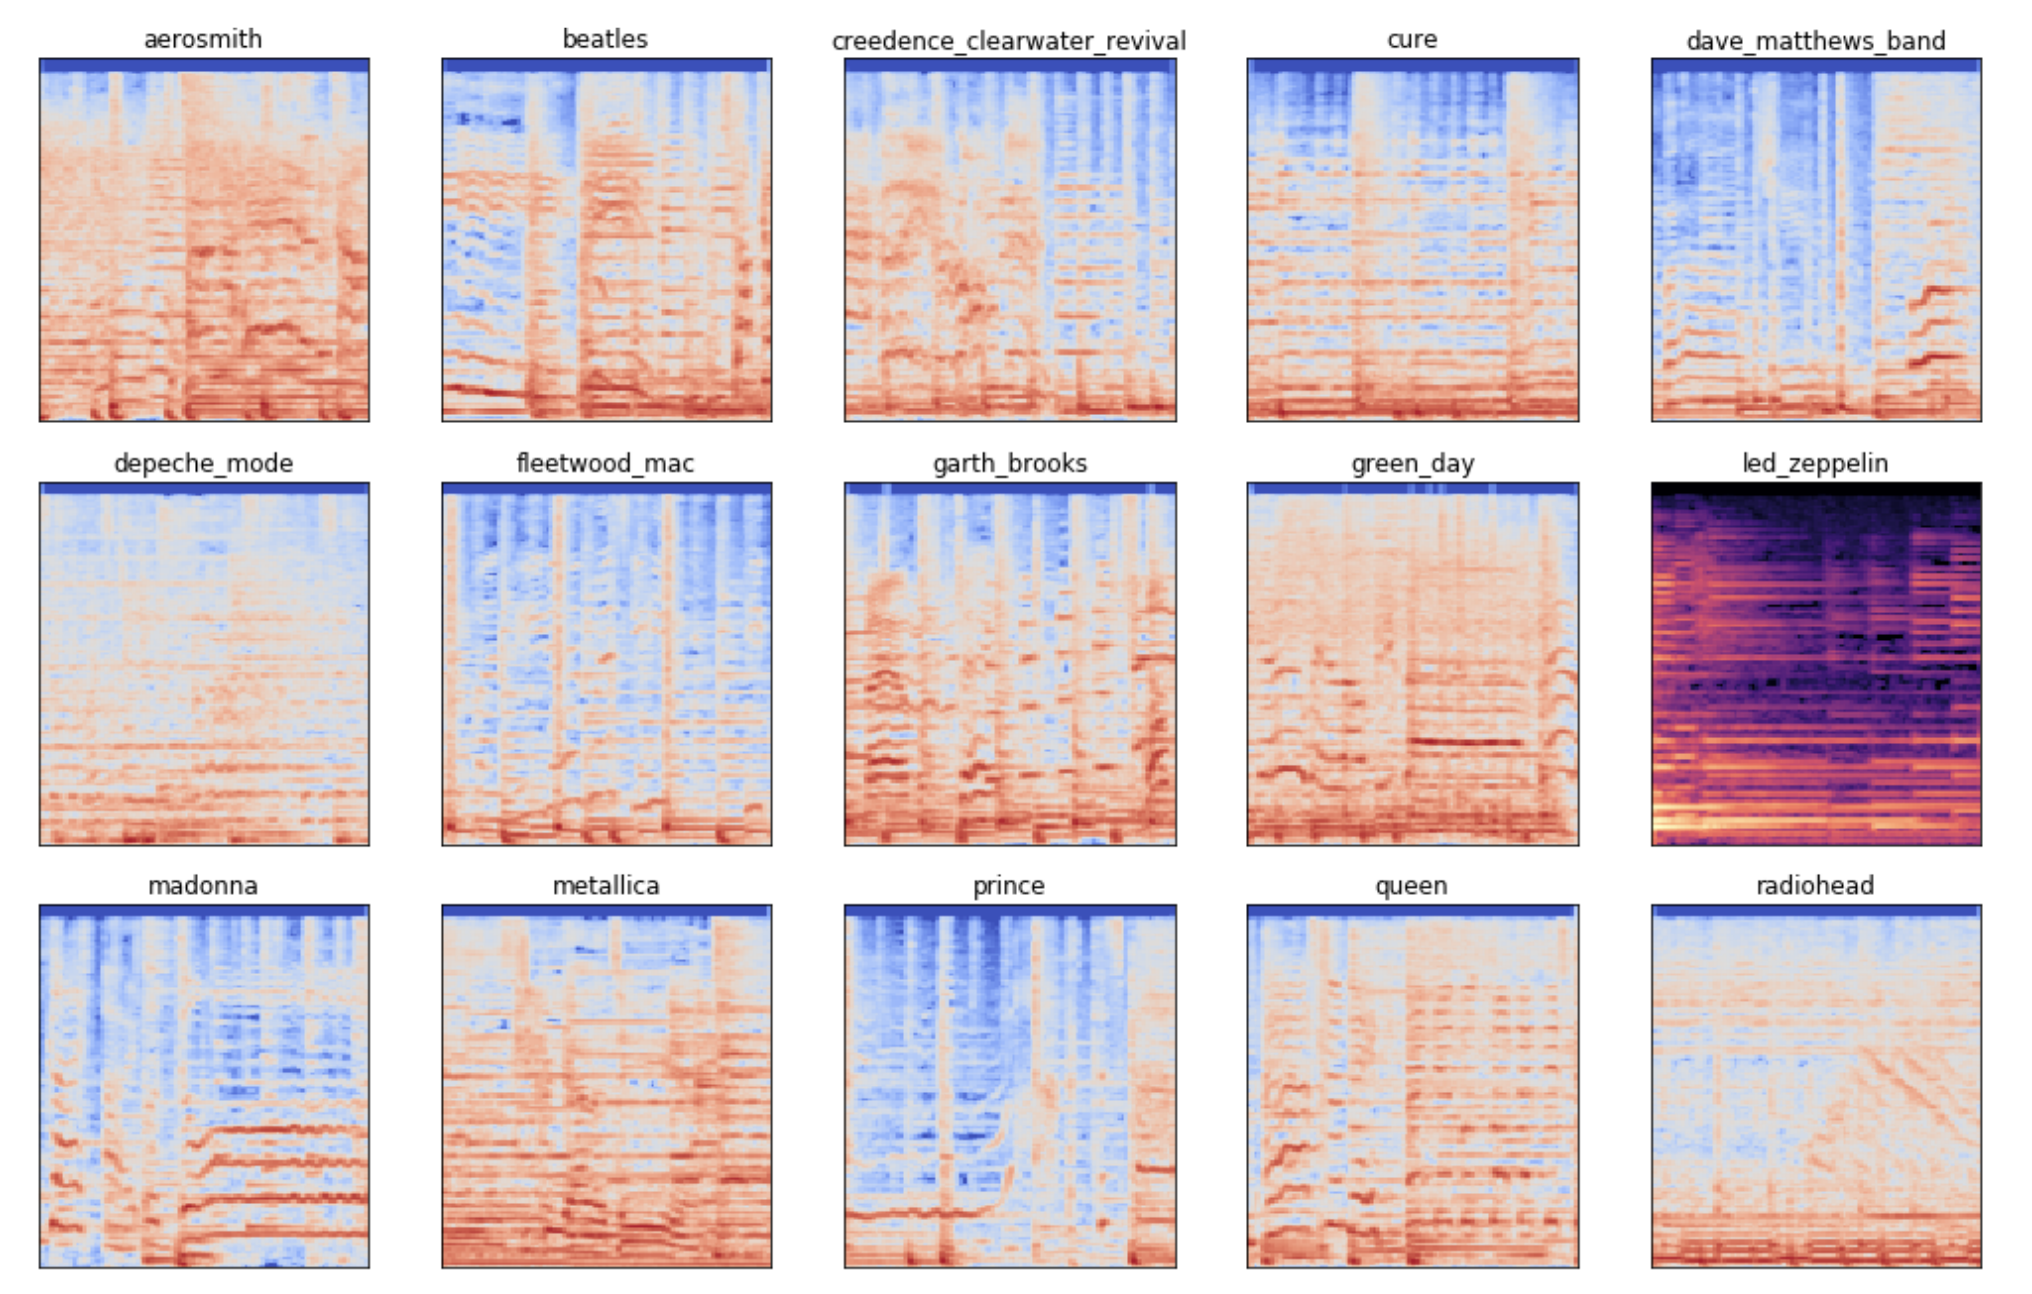
\includegraphics[width=0.7\linewidth]{img/mel.png}}
	\caption{Примеры визуализации спектрограмм композиций популярных исполнителей}
	\label{fig:spec}
\end{figure}

Возможность представить основные характеристики аудиоданных в виде изображения позволяет применить существующие практики
нейросетевого анализа изображений для анализа и классификации аудиозаписей \cite{cyber_alex}.
Для работы с изображениями зачастую применяются сверточные нейронные сети (CNN), также известные как конволюционные нейронные сети.

Свёрточная нейронная сеть — специальная архитектура искусственных нейронных сетей, предложенная Яном Лекуном в 1988 году и нацеленная на эффективное распознавание образов, входит в состав технологий глубокого обучения. 
Использует некоторые особенности зрительной коры, в которой были открыты так называемые простые клетки, реагирующие на прямые линии под разными углами, и сложные клетки, реакция которых связана с активацией определённого набора простых клеток. 

Таким образом, идея свёрточных нейронных сетей заключается в чередовании свёрточных слоёв и субдискретизирующих слоёв. Структура сети — однонаправленная (без обратных связей), принципиально многослойная. Для обучения используются стандартные методы, чаще всего метод обратного распространения ошибки. Функция активации нейронов (передаточная функция) — любая, по выбору исследователя.

Название архитектура сети получила из-за наличия операции свёртки, суть которой в том, что каждый фрагмент изображения умножается на матрицу (ядро) свёртки поэлементно, а результат суммируется и записывается в аналогичную позицию выходного изображения. 

Сверточные нейронные сети (СНС) обладают большей временной эффективностью в сравнении с перцептроном, так как необходимо
работать с меньшим количеством параметров. СНС также лучше выделяют отдельные элементы изображения (углы,
кривые, прямые, яркие области и т. д.) за счет использования нескольких карт признаков на одном слое, а также могут 
выделять высокоуровневые признаки на основе низкоуровневых \cite{cyberbred}.

Ключевым элементом сверточных нейронных сетей является ядро, которое позволяет уменьшить размерность входных данных.
Например, если исходными данными является матрица размера $M\times N$, то при использовании ядра размера $mn$ результатом свертки будет
матрица размера $(M-m+1)\times(N-n+1)$ \cite{cyberbred}.

Данный результат достигается тем, что мы "скользим" по подматрицам исходной матрицы, применяя на них преобразование свертки,
в результате чего из элементов исходной матрицы $I$ получается новая матрица $O$ меньшей размерности следующим образом:
\begin{equation}
	O_{x,y} = \sum_{i,j} W_{i,j} \sum_{\substack{t,k\\\left|t-i\right|<l\\ \left|k-j\right|<l} } I_{t,k},
\end{equation}
где 
$I$ — входные данные, $O$ — выходные, также называемые картой признаков, $W$ — ядро свертки, $l$ — коэффициент расширения. 

Для уплотнения карты признаков применяется слой пулинга (иначе подвыборки, субдискретизации), который представляет собой нелинейное уплотнение карты признаков, при этом группа пикселей (обычно размера 2×2) уплотняется до одного пикселя, проходя нелинейное преобразование. Наиболее употребительна при этом функция максимума. Преобразования затрагивают непересекающиеся прямоугольники или квадраты, каждый из которых ужимается в один пиксель, при этом выбирается пиксель, имеющий максимальное значение. Операция пулинга позволяет существенно уменьшить пространственный объём изображения. Пулинг интерпретируется так: если на предыдущей операции свёртки уже были выявлены некоторые признаки, то для дальнейшей обработки настолько подробное изображение уже не нужно, и оно уплотняется до менее подробного. К тому же фильтрация уже ненужных деталей помогает не переобучаться. Слой пулинга, как правило, вставляется после слоя свёртки перед слоем следующей свёртки.
Кроме пулинга с функцией максимума можно использовать и другие функции — например, среднего значения или $L_2$-нормирования. Однако практика показала преимущества именно пулинга с функцией максимума, который включается в типовые системы \cite{wikiconv}. 

\chapter{Кластеризация и классификация аудиоданных при помощи нейронных сетей}
Для демонстрации работы нейросетевых методов анализа аудиоданных предлагается провести классификацию музыкальных композиций
по заранее определенным жанрам. В рамках данной работы была подготовлена выборка музыкальных композиций 4 жанров различного происхождения:
Phonk -- поджанра американской хип-хоп музыки, Intelligent dance music (IDM), классической музыки и Neofolk. Каждому жанру в среднем отведено 100 композиций, что соизмеримо с другими наборами данных, предназначенных для аналогичных исследований \cite{gtzan}.

Для удобства подготовки данных, предназначенных для обучения, также был написан модуль, который позволяет подготавливать датасет композиций
с заранее заданной длиной и выделением характеристик при помощи библиотеки работы со звуком Librosa \cite{librosa}. Для сравнения был подготовлен набор данных из
композиций продолжительностью 30 секунд и выделением характеристик: оконное преобразование Фурье (STFT), мел-кепстральные коэффициенты (MFCC), спектрограмма, Tonnetz, спектральные показатели контрастности и хроматограмма по оконному преобразованию Фурье.  Вышеупомянутая характеристика Tonnetz в русскоязычной литературе зачастую фигурирует как тональный центроид.

%TODO
Для первичной классификации жанров при составлении датасета был использован рекомендательный сервис музыки Last.fm, который также используется в других исследованиях, \cite{lastfm}, который
формирует связи между композициями и жанрами, исходя из предоставляемой пользователями статистики прослушивания.
Часть данных из датасета используем для обучения нейронных сетей, 
а часть используем как входные данные для анализа обученной нейросетью. 

В данном исследовании будет проведено сравнение
нейросетей, обученных с учителем и без. В качестве примера обучения без учителя приводится aлгоритм K-Means.
K-Means базируется на идее минимизации функции:
\begin{equation}
	J = \sum_{j=1}^k \sum_{x \in S_i}^n \left|\left| x - c_j\right|\right|^2,
\end{equation}
где $S_i$ -- кластеры, $k$ -- число кластеров $c_j$ -- центры кластеров.

Алгоритм представляет собой версию EM-алгоритма, применяемого также для разделения смеси гауссиан. Он разбивает множество элементов векторного пространства на заранее известное число кластеров k.
Основная идея заключается в том, что на каждой итерации перевычисляется центр масс для каждого кластера, полученного на предыдущем шаге, затем векторы разбиваются на кластеры вновь в соответствии с тем, какой из новых центров оказался ближе по выбранной метрике.
Алгоритм завершается, когда на какой-то итерации не происходит изменения внутрикластерного расстояния. Это происходит за конечное число итераций, так как количество возможных разбиений конечного множества конечно, а на каждом шаге суммарное квадратичное отклонение V уменьшается, поэтому зацикливание невозможно.

В качестве примера алгоритма обучения с учителем предлагается использовать нейронную сеть с одним входным слоем, одним скрытым и одним выходным слоем на базе фреймворка машинного обучения tensorflow \cite{tensorflow}.
Архитектура нейронной сети и ее конфигурация задается моделью, которая складывается из слоев. 
Данный фреймворк также предоставляет встроенные оптимизаторы процесса обучения сети, которые позволяют уменьшить погрешность модели за счет минимизации некоторых ее параметров. В рамках данного исследования будем использовать оптимизатор Adam, представленный в 2014 году, который основан на идее градиентного бустинга \cite{adam}.

Градиентный бустинг -- это техника машинного обучения, которая применеяется для улучшения результатов в задачах классификация. Идея состоит в минимазации функции потерь $L(y, y^p)$, которая может быть определена в среднеквадратичном смысле (MSE) следующим образом:
\begin{equation}
	L(\hat y) = \sum_{i} (y_i - \hat y _i)^2,
\end{equation} 

где $y_i$ -- это это целевое значние, а $\hat y_i$ --предположение сделанное нейронной сетью.
Для улучшения точности предположений нейронной сети необходимо подобрать $\hat y_i$ так, чтобы они были близки к $y_i$, что сводится к задаче численного нелинейного программирования.
Для этого значение $k$-ого приближения $\hat y_i^k$ полагают равным:

\begin{equation}
	\hat y_i^k =\hat y_i^{k-1} - \alpha \frac{\partial L(\hat y)}{\partial \hat y_i},
\end{equation}
где $\alpha$ -- это шаг, с которым подбирается приближение. В задачах обучения нейронных сетей его иногда полагают скорости обучения сети.


\chapter{Сравнение полученных результатов с априорной классификацией}

Для определения погрешности модели на основе обучения с учителем применим встроенные инструменты фреймворка tensorflow.
Модель, обученная на 100 эпохах, демонстрирует 0.78\% процентную точность на тестовых данных. В некоторых источниках приводится также точность модели на элементах выборки для обучения. В данном случае она составила 100\%, хотя особенного интереса это представляет.


В контексте данной данной задачи разбиение на кластеры музыкальных композиций будет определять ее принадлежность к соответствующим жанрам.
Для удобства программной реализации при подготовке данных метки принадлежности к жанру
будем хранить, как целые числа от 0 до 3. В связи с этим возникает проблема оценки эффективности
разбиения выборки для обучения на жанры, так как в процессе применения алгоритма K-Means кластерам
присвоятся метки кластеров вне зависимости от априорной классификации. Поэтому в качестве показателя эффективности
кластеризации будем использовать максимум по всем возможным соответствиям априорной классификации к меткам кластеризации, т.е.
\begin{equation}
	1 - \varepsilon = \underset{(i,j) \in (0, \dots, k)^2}{\max} \frac{1}{\left|\mathbb{X}\right|}\sum_{i=1}^n \varphi(x_i),
\end{equation}
где
	$$\varphi(x) = 
	\begin{cases}
		1, &  x \in S_i \wedge x \in A_i \\
		0, & \text{в ином случае}
	\end{cases}, $$
	$S_i$ -- разбиение выборки на кластеры, а $A_i$ -- ариорное разбиение выборки.
Другими словами, выберем такое соответствие меток исходного набора данных к меткам, используемым KMeans, чтобы ошибка классификации -- отношение неправильно классифицированных композиций к общему числу композиций -- была минимальной.

Итого, точность, полученная при использовании данного подхода, составила $0.43$\%, что гораздо ниже, чем точность, полученная при использовании нейронной сети, обученной на метках с данными о жанрах.

\chapter{Общие результаты и выводы}

Использование алгоритмов обучения с привлечением учителя показало лучший результат по сравнению с алгоритмом обучения без учителя.